\documentclass{scrartcl}
\usepackage{handout}
\usepackage{pgfplots,pgf-pie, multirow}
\pgfplotsset{compat=1.18}
\usepackage{tikz}

\setlength{\tabcolsep}{10pt}
\setlength{\arrayrulewidth}{0.6pt}
\renewcommand{\arraystretch}{1.175}

\title{Lab Report Prey Predator Dynamics}
\author{Piyush Kumar Singh (22MS027)\\Sabarno Saha (22MS037)\\Diptanuj Sarkar (22MS038)}
\date{}

\begin{document}
\maketitle
\tableofcontents
\newpage

\section{Data}

\subsection{Prey Population}
\begin{table}[H]
    \centering
    \begin{tabular}{|l|c|c|c|c|c|c|c|}
        \hline
        {} & \multicolumn{7}{c|}{Prey at start of Generation} \\
        \cline{2-8}
        {} & 1 & 2 & 3 & 4 & 5 & 6 & 7 \\
        \hline \hline
        Prey 1: White Bean & 20 & 24 & 30 & 51 & 141 & 414 & 1239\\ 
        \hline
        Prey 2: Black Bean & 20 & 51 & 99 & 255 & 735 & 2115 & 6246\\
        \hline
        Prey 3: Pasta & 20 & 12 & 20 & 30 & 48 & 84 & 154\\
        \hline
    \end{tabular}
    % \label{tab:my_label}
\end{table}


\subsection{Prey after each generation}
\begin{table}[H]
    \centering
    \begin{tabular}{|l|c|c|c|c|c|c|c|}
        \hline
        {} & \multicolumn{7}{c|}{Prey Remaining} \\
        \cline{2-8}
        {} & 1 & 2 & 3 & 4 & 5 & 6 & 7 \\
        \hline \hline
        Prey 1: White Bean & 8 & 10 & 17 & 47 & 138 & 413 & 1227\\ 
        \hline
        Prey 2: Black Bean & 17 & 33 & 85 & 245 & 705 & 2082 & 6234\\
        \hline
        Prey 3: Pasta & 6 & 10 & 15 & 24 & 42 & 77 & 136\\
        \hline
    \end{tabular}
    % \label{tab:my_label}
\end{table}


\subsection{Prey consumed by Predator (Knives/Mouth)}
\begin{table}[H]
\centering
\begin{tabular}{|l|c|c|c|c|c|c|c|}
\hline
    \multirow{2}{*}{Mouth (Knives)} & \multicolumn{7}{c|}{Prey consumed by Predator} \\
    \cline{2-8}
     & 1 & 2 & 3 & 4 & 5 & 6 & 7 \\
    \hline \hline
    Prey 1: White Bean & 2 & 4 & 7 & 2 & 1 & 1 & 5\\ 
    \hline
    Prey 2: Black Bean & 0 & 2 & 1 & 4 & 7 & 10 & 4\\
    \hline
    Prey 3: Pasta & 5 & 1 & 0 & 0 & 0 & 0 & 0\\
    \hline
    Total:        & 0 (Poisoned) & 7 & 6 & 8 & 6 & 11 & 9\\
    \hline
\end{tabular}
\end{table}

\subsection{Prey consumed by Predator (Spoons/Raptorial)}
\begin{table}[H]
\centering
\begin{tabular}{|l|c|c|c|c|c|c|c|}
\hline
    \multirow{2}{*}{Raptorial (Spoons)} & \multicolumn{7}{c|}{Prey consumed by Predator} \\
    \cline{2-8}
     & 1 & 2 & 3 & 4 & 5 & 6 & 7 \\
    \hline \hline
    Prey 1: White Bean & 6 & 3 & 0 & 0 & 0 & 0 & 0\\ 
    \hline
    Prey 2: Black Bean & 3 & 7 & 0 & 0 & 0 & 0 & 0\\
    \hline
    Prey 3: Pasta & 4 & 1 & 5 & 6 & 6 & 7 & 8\\
    \hline
     Total:       & 0 (Poisoned) & 11 & 5 & 6 & 6 & 7 & 8\\
     \hline
\end{tabular}
\end{table}

\subsection{Prey consumed by predator(Fork/Legs)}

\begin{table}[H]
\centering
\begin{tabular}{|l|c|c|c|c|c|c|c|}
\hline
    \multirow{2}{*}{Legs (Forks)} & \multicolumn{7}{c|}{Prey consumed by Predator} \\
    \cline{2-8}
    & 1 & 2 & 3 & 4 & 5 & 6 & 7 \\
    \hline \hline
    Prey 1: White Bean & 4 & 7 & 6 & 2 & 2 & 0 & 7\\ 
    \hline
    Prey 2: Black Bean & 0 & 9 & 11 & 6 & 23 & 23 & 8\\
    \hline
    Prey 3: Pasta & 5 & 0 & 0 & 0 & 0 & 0 & 0\\
    \hline
    Total:        & 0 (Poisoned) & 16 & 17 & 8 & 25 & 23 & 15\\
    \hline
\end{tabular}
\end{table}

\section{Data Analysis}

\subsection{Population Growth of Prey}

\subsubsection{Population Analysis of White Bean}
\begin{center}
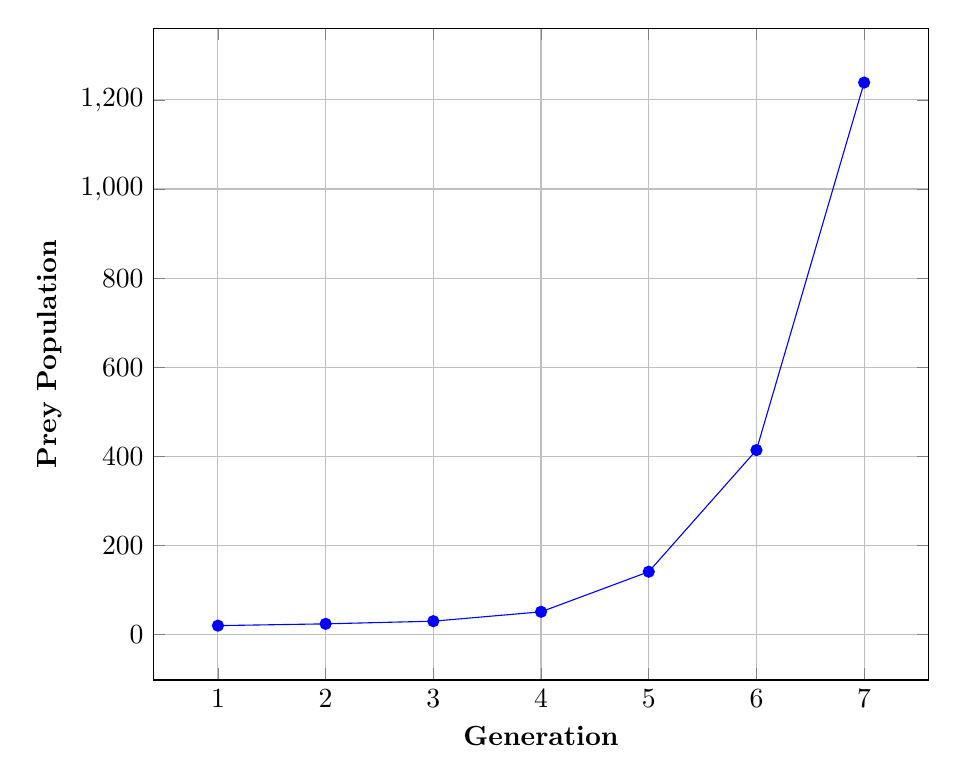
\begin{tikzpicture}
	\begin{axis}[
    width =4.5 in,
		xlabel=\textbf{Generation},
		ylabel=\textbf{Prey Population},
        grid=major,
        xtick={1,2,3,4,5,6,7},
        ytick={0,200,400,600,800,1000,1200,1400}]
	\addplot[color=blue,mark=*] coordinates {
		(1,20)
		(2,24)
        (3,30)
		(4,51)
		(5,141)
		(6,414)
		(7,1239)
	};
	\end{axis}
\end{tikzpicture}
\end{center}

The population of the white bean grew exponentially in the system, but they did not form the most significant population at the end of the experiment. Due to the intermediate size of the beans, they were reasonably easy for all the predators to pick up. 

\subsubsection{Population Analysis of Black Bean}
\begin{center}
    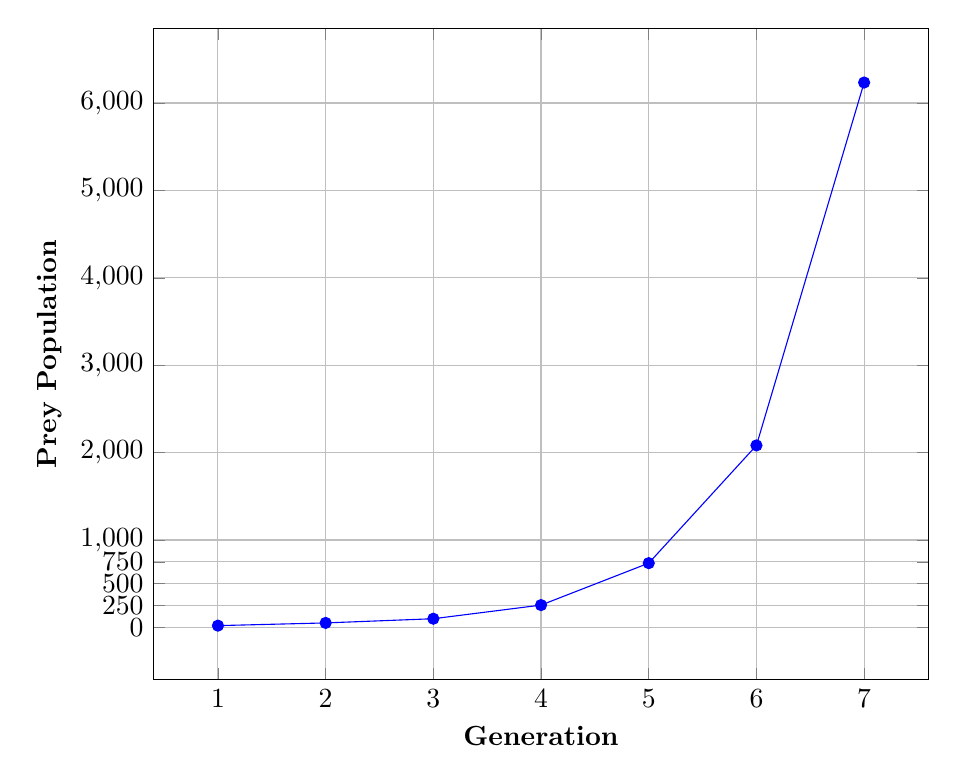
\begin{tikzpicture}
	\begin{axis}[
    width =4.5 in,
		xlabel=\textbf{Generation},
		ylabel=\textbf{Prey Population},
        grid=major,
        xtick={1,2,3,4,5,6,7},
        ytick={0,250,500,750,1000,2000,3000,4000,5000,6000,7000}]
	\addplot[color=blue,mark=*] coordinates {
		(1,20)
		(2,51)
        (3,99)
		(4,255)
		(5,735)
		(6,2082)
		(7,6234)
	};
	\end{axis}
\end{tikzpicture}
\end{center}

The black bean population grew exponentially, forming the largest prey population at the end of the experiment. The small size of the beans made it challenging to pick up for the predators like the knives (mouth) and the spoons (raptorial) predators. This allowed it to grow to such a large size.

% \vocab{Continued on next page...}

\subsubsection{Population Analysis of Pasta}
\begin{center}
   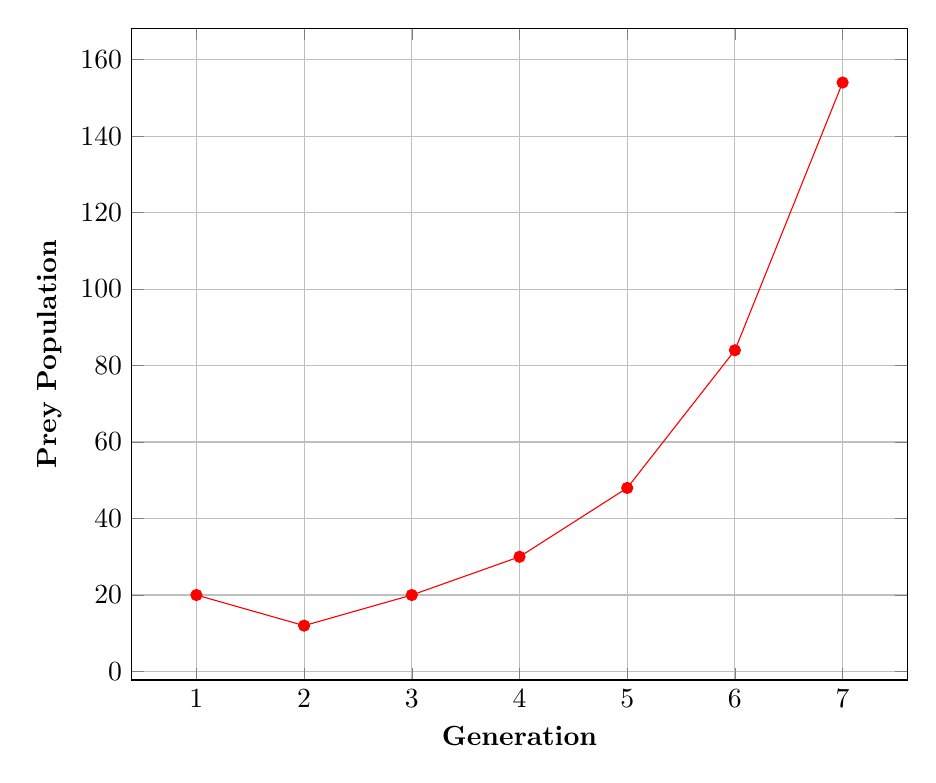
\begin{tikzpicture}
	\begin{axis}[
    width =4.5 in,
		xlabel=\textbf{Generation},
		ylabel=\textbf{Prey Population},
        grid=major,
        xtick={1,2,3,4,5,6,7}]
	\addplot[color=red,mark=*] coordinates {
		(1,20)
		(2,12)
        (3,20)
		(4,30)
		(5,48)
		(6,84)
		(7,154)
	};
	\end{axis}
\end{tikzpicture} 
\end{center}

The population of pasta fell initially, as it was large and easy to pick up using all of the three different kinds of appendages available. But after the realization of the toxicity of the pasta, all predators except the raptorial predator stopped consuming it. This allowed the population of pasta to increase. Due to the reduced reproductive ability of the pasta, their numbers did not increase to the magnitudes reached by the white and black bean populations.

\subsection{Prey Preference of each Predator}
\subsubsection{Predator using Knives(Mouth)}
\begin{center}
    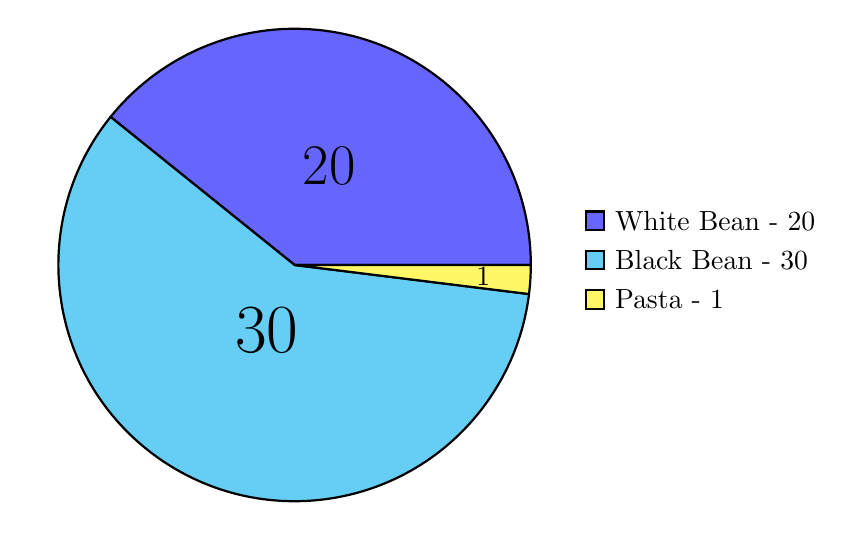
\begin{tikzpicture} 
    \pie[sum =51,scale font, radius = 3,text=legend]{20/White Bean - 20,30/Black Bean - 30,1/Pasta - 1} 
\end{tikzpicture}
\end{center}
% \pagebreak
This predator had difficulty in picking up prey due to the shape of its appendages, but it eventually managed to sustain itself on the abundant populations of white and black beans in the environment. This predator was the second most successful, with a total of 51 prey consumed out of 198.
\textcolor{red!80!black}{$$\fbox{$
\frac{\text{No. of prey consumed}}{\text{total prey consumed by all predators}} = \frac{51}{198}
$}$$}

\subsubsection{Predator using Spoons(Raptorial)}
\begin{center}
    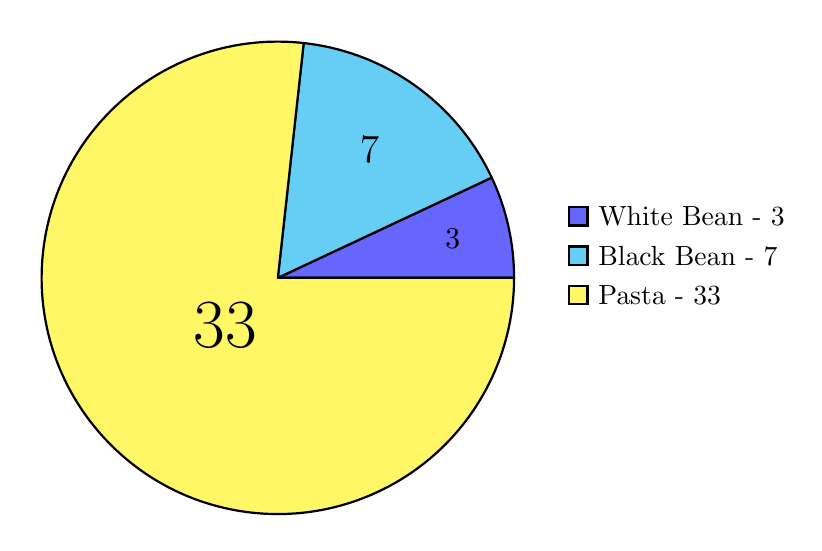
\begin{tikzpicture} 
    \pie[sum =43,scale font, radius = 3,text=legend]{3/White Bean - 3,7/Black Bean - 7,33/Pasta - 33} 
\end{tikzpicture}
\end{center}

This predator was the least successful, with a total of 43 prey eaten out of 198. It could capture prey easily due to the shape of its appendages, but it preferred to consume pasta almost exclusively after it discovered its natural resistance to the toxicity of pasta - possibly because of no competition in consuming pasta. Due to the large size of the pasta, it was able to capture a lesser amount of prey than the other predators in one go and consumed just a little more than what was required to sustain itself.
\textcolor{red!80!black}{$$\fbox{$
\frac{\text{No. of prey consumed}}{\text{total prey consumed by all predators}} = \frac{43}{198}
$}$$}

\subsubsection[\textcolor{purple}{The Most Successful Predator}]{Predator using Forks(Legs)}
\begin{center}
    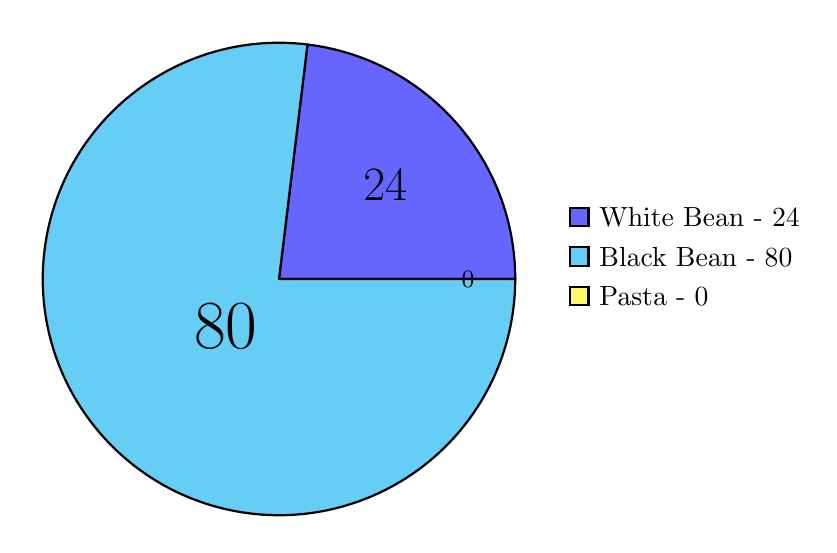
\begin{tikzpicture} 
    \pie[sum =104,scale font, radius = 3,text=legend]{24/White Bean - 24,80/Black Bean - 80,0/Pasta - 0} 
\end{tikzpicture}
\end{center}

\vocab{This predator was the most successful}, having consumed a total of 104 prey out of 198. It preferred black beans as they were smaller and easier to capture using its leg appendages.
\textcolor{red!80!black}{$$\fbox{$
\frac{\text{No. of prey consumed}}{\text{total prey consumed by all predators}} = \frac{104}{198}
$}$$}
% \begin{center}
%     \fbox{This Predator was the most successful}
% \end{center}

% \pagebreak
\section{Questions}
\begin{question}
    When a potential prey becomes toxic, what happens to the number of prey individuals of this population initially? Will their numbers increase indefinitely?
\end{question}

\begin{solution*}
Initially, the reproductive rate of the potential prey species decreases due to the individuals of the species expending more energy/resources in producing the toxin. But due to the lower rates of predation owing to the toxin, the population size increases until one or more species develop resistance to the toxin and become specialized predators.
\end{solution*}

\begin{question}
    What happens when prey reproduce more quickly than that can be controlled by predators? What other factors control populations?
\end{question}

\begin{solution*}
If prey reproduces faster than what can be controlled via consumption by predators, the population size of the prey species will keep increasing until it reaches a size where the environment itself can not support it anymore, i.e. the carrying capacity. Factors that cause this are several and mainly include the limited amount of resources and habitats available for the prey species.    
\end{solution*}

\begin{question}
    What would happen if the environment was affected by chance events like cyclones or drought? Which of the species (Specialist or generalist) will survive and why?
\end{question}

\begin{solution*}
If the environment was affected by a sudden natural disaster like a cyclone or a drought, the population sizes of all the prey species would be diminished by roughly the same amount. In this case, the generalist predator will survive with greater ease as it can consume individuals of all prey species. It will have a larger pool of prey to survive on compared to the specialist, who will now have an even smaller number of prey individuals in the species they consume. In such a scenario, the specialist predator might even go extinct if the prey it specializes in reduces significantly in number.
\end{solution*}

\begin{question}
    Did all predator and prey types remain in the environment in your experiment? Or was your environment reduced to two species? If yes, then give reasons why this could have happened.
\end{question}

\begin{solution*}
Yes, all the predator and prey types remained alive in the environment throughout our experiment. The predators were unable to consume the prey at a rate that compared to the reproductive rates of the prey species, and as a result, the population sizes of all the prey species grew greatly in number. In turn, this overabundance of prey individuals sustained all the predators adequately for all 7 rounds of the experiment, and no-one went extinct.
\end{solution*}

\end{document}
